% !TEX root = tracking.tex
\section{Introduction}

When it comes to autonomous dynamical systems, safety and real-time planning are both crucial for many worthwhile applications.
This is particularly true when environments are \textit{a priori} unknown, because replanning based on updated information about the environment is often necessary. 
%Autonomous systems have a great potential to improve many industries in the near future. 
%To be most effective in these endeavors it is useful for systems to make real-time plans while maintaining safety guarantees.
%However, to achieve this potential there is a need to ensure the ability to make real-time plans while maintaining safety guarantees.
% As unmanned aerial vehicles (UAVs) and other autonomous systems become more commonplace, it is essential that they be able to plan safe motion paths through crowded environments in real-time. 
%This is particularly crucial for navigating through environments that are \textit{a priori} unknown, because replanning based on updated information about the environment is often necessary. 
However, achieving safe navigation in real time is difficult for many common dynamical systems due to the computational complexity of generating and formally verifying the safety of dynamically feasible trajectories.
 In order to achieve real-time planning, many algorithms use highly simplified model dynamics or kinematics to create a nominal trajectory that is then tracked by the system using a feedback controller such as a linear quadratic regulator (LQR).  These nominal trajectories may not be dynamically feasible for the true autonomous system, resulting in a tracking error between the planned path and the executed trajectory.
 This concept is illustrated in Fig. \ref{fig:chasing}, where the path was planned using a simplified planning model, but the real dynamical system cannot track this path exactly. 
Additionally, external disturbances (e.g. wind) can be difficult to account for using real-time planning algorithms, causing another source of tracking error. 
These tracking errors can lead to dangerous situations in which the planned path is safe, but the actual system trajectory enters unsafe regions.  Therefore, real-time planning is achieved at the cost of guaranteeing safety.  Common practice techniques augment obstacles by an ad hoc safety margin, which may alleviate the problem but is performed heuristically and therefore does not guarantee safety.
 \begin{figure}
 	\centering
 	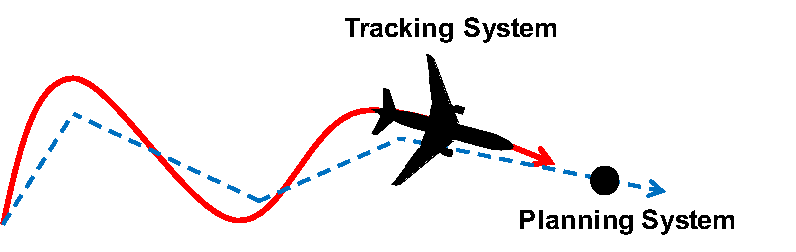
\includegraphics[width=0.7\columnwidth]{fig/chasing}
 	\caption{Left: A planning algorithm uses a fast but simple model (blue disk), to plan around obstacles (gray disks). The more complicated tracking model (green plane) tracks the path. By using FaSTrack the autonomous system is guaranteed to stay within some TEB (black circle). Right: Safety can be guaranteed by planning with respect to obstacles augmented by the TEB (large black circles).}
 	\label{fig:chasing}
 \end{figure}
 %Real-time planning that is both safe and accurate presents a very difficult challenge: accuracy and robustness in many dyanimcal systme sis difficult to compute, often precluding real-time computer hands.fast planning is generally at odds with the need for maintaining safety and robustness.  

To attain fast planning speed while maintaining safety, we propose the modular framework FaSTrack: Fast and Safe Tracking.  As before, FaSTrack allows planning algorithms to use a simplified model of the system in order to operate in real time using augmented obstacles.  However, the bound for augmenting obstacles is rigorously computed and comes with a corresponding optimal tracking controller. Together this bound and controller guarantee safety for the autonomous system as it tracks the simplified plans (see Fig. \ref{fig:chasing}, right).  

We compute this bound and controller by modeling the navigation task as a pursuit-evasion game between a sophisticated \textit{tracking model} (pursuer) and the simplified \textit{planning model} of the system (evader). 
The tracking model accounts for complex system dynamics as well as bounded external disturbances, while the simple planning model enables the use of real-time planning algorithms. 
Offline, the pursuit-evasion game between the two models can be analyzed using any suitable method \cite{Mitchell05, SinghChenEtAl2018, royo2018classification}. 
This results in a \textit{tracking error function} that maps the initial relative state between the two models to the \textit{tracking error bound} (TEB): the maximum possible relative distance that could occur over time. 
This TEB can be thought of as a ``safety bubble" around the planning model of the system that the tracking model of the system is guaranteed to stay within.

The resulting TEB from this precomputation may converge to an invariant set (i.e. the planning model cannot move arbitrarily far away from the tracking model when both act optimally), or may result in a time-varying set.
%Since the planning model can be designed by the user, typically one can select a model such that the computation converges.  
%However, there may be cases in which convergence doesn't occur (i.e. even when acting optimally the autonomous sytem cannot keep up with the planning model used by the path or trajectory planning algorithm).  In these cases we can instead compute a time-varying TEB.  
Intuitively, a time-varying TEB means that as time progresses the tracking error bound increases by a known amount.

Because the tracking error is bounded in the relative state space, we can precompute and store the \textit{optimal tracking controller} that maps the real-time relative state to the optimal tracking control action for the tracking model to pursue the planning model. 
The offline computations are \textit{independent} of the path planned in real time.

Online, the autonomous system senses local obstacles, which are then augmented by the TEB to ensure that no potentially unsafe paths can be computed. 
Next, any chosen path or trajectory planning algorithm uses the simplified planning model and the local environment to determine the next planning state. 
The autonomous system (represented by the tracking model) then finds the relative state between itself and the next desired state. 
If this relative state is nearing the TEB then it is plugged into the optimal tracking controller to find the instantaneous optimal tracking control of the tracking model required to stay within the error bound; otherwise, any tracking controller may be used. In this sense, FaSTrack provides a \emph{least-restrictive} control law.
This process is repeated for as long as the planning algorithm (rapidly-exploring random trees, model predictive control, etc.) is active. 

\MCnote{
FaSTrack is designed to be modular, and can be used with any method for computing the TEB in conjunction with any existing path or trajectory planning algorithms.  
This enables motion planning that is real-time, guaranteed safe, and dynamically accurate. 
FaSTrack was first introduced in conference form \cite{herbert2017fastrack}, and is expanded upon here in a number of important ways.
}

\MCnote{
First, we adopt definitions in \cite{} to refine the notion of relative system to be much more general; in particular, the new definition of relative state allows the pairing of a large class of tracking and planning models.
}

\MCnote{
Next, we introduce and prove the time-varying formulation of FaSTrack, which uses time-varying tracking controllers to provide a time-varying TEB (tvTEB).
This has significant practical impact, since the ability to obtain a tvTEB means that the FaSTrack framework does not depend on the convergence of pursuit-evasion games, which in general not guaranteed, computationally expensive to check, not theoretically fully understood for heterogeneous agents. 
In addition, even when the TEB is computed using other computational methods such as SOS \cite{}, obtaining a time-varying TEB is much more challenging.
}

\MCnote{
Furthermore, for both the time-invariant and time-varying cases, we provide mathematical proofs.
}

\MCnote{
Lastly, we demonstrate the FaSTrack framework by using three different real-time planning algorithms that have been ``robustified" by precomputing the TEB and tracking controller to demonstrate our contributions. 
}

\MCnote{
Precomputation of the TEB and optimal tracking control function for each planning-tracking model pair is done by solving a Hamilton-Jacobi (HJ) partial differential equation (PDE) in this paper; we encourage readers to refer to \cite{SinghChenEtAl2018} for TEB computations using SOS optimization. 
}

\MCnote{
The planning algorithms used in our numerical examples are the fast sweeping method (FSM) \cite{Takei2013}, rapidly-exploring random trees (RRT) \cite{Kuffner2000,Kavraki1996}, and model predictive control (MPC) \cite{Qin2003,Zhang2017}. 
}

\MCnote{
In the three examples, we also consider different tracking and planning models, one of which utilizes the refined definition of relative system, and another involving a tvTEB.
}

\MCnote{
In the simulations, the system travels through a static environment with constraints defined, for example, by obstacles, while experiencing disturbances.
The constraints are only fully known through online sensing (e.g. once obstacles are within the limited sensing region of the autonomous system). 
By combining the TEB with real-time planning algorithms, the system is able to safely plan and track a trajectory through the environment in real time.} 